\chapter{Design}

There are several broad approaches to implementing an AOP framework. The ideal approach is to extend the compiler of the target language to provide built-in support. Even Though the C\# compiler from Microsoft is not open source, the alternative Mono C\# compiler is, so this is a viable option. However that would have been a pretty big undertaking, and I was not sure if I can tackle and finish it in the timeframe I wanted.

If compiler support is not an option, that leaves framework support as another viable option. There are several approaches to implement framework to provide AOP capabilities.

Early on I have narrowed them down to between Runtime Interception and Compile Time Weaving. As its name suggested, runtime interception operates while the program is in execution. It involves the use of the proxy pattern, where client communicate with the target object via a proxy, and aspects are injected to the proxy, thus enabling runtime behavior of the program to be modified. As figure~\ref{proxy_model} illustrates.

\begin{figure}[here]
  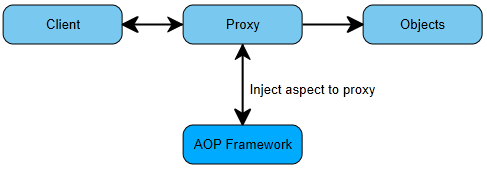
\includegraphics[scale=1.0]{Proxy.PNG}
  \centering
  \caption{AOP framework using proxy\label{proxy_model}}
\end{figure}

New functionalities can be “added” to the target object via the proxy. The disadvantage of this approach is that it involves the generation of proxy object at runtime, which will impact the runtime performance of the application. It is also restricting in that both target object and the proxy must implement a common interface for this to work, and that only virtual methods are exposed.

From the usage perspective, to set this up, a developer usually have to provide some type of mapping between the target object and the proxy via a configuration file so the actual proxy generation can occur. This approach is easier to implement, but not as easy to use.

The approach I decided to use is Compile Time Weaving. The basic idea is after compilation of the assembly, the framework takes over and disassemble the assembly, and weave in the defined aspect code to all targeted methods. This approach is more difficult to implement as it involves modifying MSIL instructions. But the advantage is that no runtime performance of proxy generation will be needed. And since this happens post compilation we can hook it into the Microsoft Build System to have the weaving invoked automatically if needed, so no manual setup is required from the developer.

Figure~\ref{buffalo_model} shows an overview of the compilation process and where Buffalo will fit in.

\begin{figure}[here]
  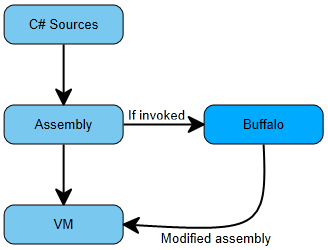
\includegraphics[scale=1.0]{BuffaloOverview.PNG}
  \centering
  \caption{AOP framework using proxy\label{buffalo_model}}
\end{figure}

\section{Method Boundary Aspect}
I also have to decide on what functionality I want to support in the framework. What kind of aspect do I want to weave into the IL instructions of the executing program? For this I took inspiration from AspectJ and PostSharp, specifically I want to intercept the various point of an executing method. Those points are namely: before a method executes; after a method executes; whether or not the method executed successfully without error; or whether the method throws an exception any point during the execution.

If we think about it, these points can be nicely mapped to the try-catch-finally statements of the .NET languages. As far as the Common Language Runtime (CLR) is concern, try-catch can be used liberally without serious performance degradation. For example, we can transform the following method:

\begin{lstlisting}[caption={Sample function}, label=samplefunction]
public void SomeFunction () {
   //Perform some action...
}
\end{lstlisting}

With something like the following, which will capture exactly what I have in mind:

\begin{lstlisting}[caption={Sample try-cath-finally}, label=sampletcf]
public void SomeFunction () {
   try {
       OnBefore();
       //Perform some action
       OnSuccess();
   }
   catch (Exception e) {
       OnException(e);
   }
   finally {
       OnAfter();
   }
}
\end{lstlisting}

The above transformed method still does what the original method intends to do, only now at various point execution are being intercepted. I call these various point of interception the MethodBoundaryAspect.

\section{Method Around Aspect}
Another type of aspect that Buffalo implemented is the MethodAroundAspect. Rather than intercepting various execution point, I can also completely replace a target method with some other method defined in an aspect. While preserving the option to call back into the original method if necessary.

At first glance MethodAroundAspect sounds straightforward to do, but it turns out to be much more involved than the MethodBoundaryAspect.

Since the option to call back into the original method is preserved, that means I can under no way modify the original method. If I simply yank out its method body instructions and replace them with my own, the call back to the original method will be meaningless since the method is now not the original method. The original method must be intact for the call back to happen.

That leads me to dynamically generating a method in MSIL with the same method signature as the original.

In this generated method I issued a call to the aspect’s Invoke() method, which is the actual aspect code I want to run. Inside the Invoke method, developer can make a call back to the original method via a call to the Procee() method. Then throughout the program, for any calls made to the original method, I would change them to call the generated method instead. This is illustrated in figure~\ref{around_overview}

\begin{figure}[here]
  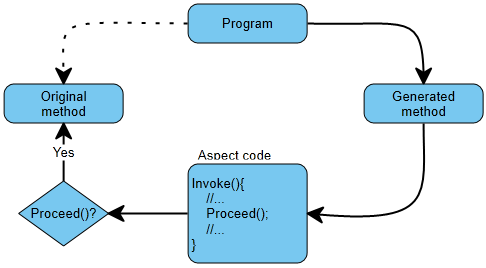
\includegraphics[scale=1.0]{AroundOverview.PNG}
  \centering
  \caption{Method Around Aspect\label{around_overview}}
\end{figure}

The dotted line from Program to the Original method indicates that, once the Around aspect is applied to it, there is now no direct call to it anymore.
